\documentclass[conference]{IEEEtran}
\usepackage[utf8]{inputenc}
\usepackage{graphicx}
\usepackage{amsmath,amssymb}
\usepackage{cite}
\usepackage{url}
\usepackage{booktabs}
\usepackage{multirow}

\begin{document}

\title{Uncertainty-Driven Learning Framework:\\Adaptive Knowledge Reasoning for\\Targeted Neural Network Retraining}

\author{
\IEEEauthorblockN{Jisto Prakash, Aflaha C, Ardhra K, Shifna A M}
\IEEEauthorblockA{Department of Computer Science and Engineering\\
Government Engineering College Palakkad, Kerala, India\\
Corresponding Author: Jisto Prakash}
}

\maketitle

% ================================================================
% ABSTRACT
% ================================================================
\begin{abstract}
Uncertainty-guided retraining---selecting high-entropy samples to update a neural network---is a widely adopted strategy for automated model correction. However, our preliminary experiments on CIFAR-10 and Fashion-MNIST indicate that blindly retraining on uncertain samples may degrade performance relative to an untouched baseline, consistent with catastrophic forgetting and decision-boundary distortion. We argue that this failure arises because existing methods answer \emph{``which samples are uncertain?''} but neglect the more fundamental question: \emph{``why is this prediction uncertain?''} We propose the \textbf{Adaptive Knowledge Reasoning Module (AKRM)}, a novel intermediate reasoning layer designed to diagnose the source of predictive uncertainty through latent-space analysis before selecting a targeted learning strategy. To prevent catastrophic forgetting during retraining, the framework employs teacher--student Knowledge Distillation as a first-class design constraint. This paper presents the motivation, preliminary observations, and architectural blueprint of AKRM as an early-stage student research contribution.
\end{abstract}

% ================================================================
% I. INTRODUCTION
% ================================================================
\section{Introduction}

The deployment of deep neural networks (DNNs) in safety-critical domains has accelerated interest in automated, uncertainty-aware model updating. Monte Carlo (MC) Dropout~\cite{gal2016dropout} and Deep Ensembles~\cite{lakshminarayanan2017simple} enable practical estimation of predictive uncertainty at inference time. A natural operational extension is uncertainty-guided retraining: selecting the highest-uncertainty samples and using them to update the model.

This strategy shares its foundation with active learning~\cite{settles2009active}, where uncertain samples are considered most informative. However, a critical distinction exists: active learning assumes a human oracle provides corrective labels for ambiguous samples. In the fully automated closed-loop setting we study, no such oracle exists. Our preliminary experiments suggest this distinction has significant practical consequences: blindly retraining on uncertain samples consistently failed to outperform an unmodified baseline and, in several configurations, measurably degraded performance. Two failure modes were observed: (i)~\textbf{catastrophic forgetting}~\cite{kirkpatrick2017overcoming}, wherein gradient updates on uncertain samples disrupted previously consolidated representations, and (ii)~\textbf{decision-boundary distortion}, reflected in increased Expected Calibration Error (ECE)~\cite{guo2017calibration}.

These observations motivate a central research question: \emph{Can neural networks correct their knowledge gaps more effectively by first reasoning about why a prediction is uncertain, rather than immediately retraining on uncertain samples?}

We introduce the \textbf{Adaptive Knowledge Reasoning Module (AKRM)}---a framework component designed to mediate between uncertainty estimation and learning. A core design decision is that catastrophic forgetting is treated as a hard constraint: all targeted retraining is performed via teacher--student Knowledge Distillation~\cite{hinton2015distilling}, wherein the frozen baseline model provides distributional anchoring to prevent knowledge overwriting during student model updates.

The preliminary contributions are:
\begin{enumerate}
    \item \textbf{Preliminary empirical observations} suggesting that direct uncertainty-guided retraining may degrade performance through catastrophic forgetting and boundary distortion.
    \item \textbf{Introduction of AKRM}, a reasoning-driven intermediate layer that hypothesises a causal structure for model uncertainty before selecting a learning strategy.
    \item \textbf{A modular architecture} that explicitly separates uncertainty estimation, gap diagnosis, and learning decision-making.
    \item \textbf{A research direction} toward reasoning-driven, uncertainty-aware continual learning.
\end{enumerate}

\subsection{Novelty Statement}
To the best of our knowledge, existing uncertainty-aware learning methods map uncertainty scores directly to retraining decisions, treating uncertainty as a final selection signal. No prior framework introduces an explicit reasoning stage between uncertainty estimation and learning. The novelty of AKRM lies not in uncertainty estimation itself---which is well-established~\cite{gal2016dropout,lakshminarayanan2017simple,gawlikowski2023survey}---but in the introduction of a structured reasoning layer that first asks \emph{``why is this prediction uncertain?''} before deciding \emph{``how should the model learn?''} This three-stage structure (estimate $\rightarrow$ diagnose $\rightarrow$ act) constitutes the primary conceptual contribution of this work.

% ================================================================
% II. RELATED WORK
% ================================================================
\section{Related Work}

\textbf{Uncertainty Estimation.}
Gal \& Ghahramani~\cite{gal2016dropout} established MC Dropout as a practical Bayesian approximation for epistemic uncertainty. Lakshminarayanan \emph{et al.}~\cite{lakshminarayanan2017simple} demonstrated that ensembling independently trained models provides robust calibration. Gawlikowski \emph{et al.}~\cite{gawlikowski2023survey} provide a comprehensive 2023 survey distinguishing epistemic from aleatoric uncertainty and identifying challenges in deploying uncertainty estimates within automated pipelines. Wang \& Ji~\cite{wang2024epistemic} propose gradient-based epistemic uncertainty quantification for pre-trained networks without model modification.

\textbf{Active Learning \& Continual Learning.}
Settles~\cite{settles2009active} surveys entropy-based and query-by-committee active learning strategies. Kirkpatrick \emph{et al.}~\cite{kirkpatrick2017overcoming} formally characterised catastrophic forgetting and proposed Elastic Weight Consolidation; their finding that targeted gradient updates overwrite consolidated representations directly motivated our distillation-based retraining design.

\textbf{Knowledge Distillation \& Calibration.}
Hinton \emph{et al.}~\cite{hinton2015distilling} introduced distillation for model compression; we adopt it specifically as a forgetting-prevention mechanism. Nguyen \emph{et al.}~\cite{nguyen2015fooled} demonstrated that DNNs assign high confidence to erroneous inputs. Guo \emph{et al.}~\cite{guo2017calibration} formalised ECE as a calibration metric used in our evaluation.

\textbf{Gap in Existing Work.}
No prior framework introduces a reasoning layer between uncertainty estimation and retraining that asks \emph{why} a sample is uncertain before deciding \emph{how} to learn from it.

% ================================================================
% III. PRELIMINARY EXPERIMENTS
% ================================================================
\section{Preliminary Experimental Observations}

\textbf{Experiment~1---Fashion-MNIST.}
A CNN was trained on Fashion-MNIST. Using MC Dropout ($T=30$ passes), predictive entropy was estimated for each training sample. The top $K=10\%$ by entropy were selected and used to augment the training set before standard offline retraining. The resulting accuracy change was marginal and inconsistent across runs, suggesting that uncertainty alone is an insufficient signal for productive model updating on a near-saturated benchmark.

\textbf{Experiment~2---CIFAR-10.}
A structured comparison across four pipelines was conducted: (A)~Baseline (no retraining), (B)~Random-sample retraining, (C)~Uncertainty-guided retraining (MC Dropout, no diagnosis), and (D)~an early AKRM prototype. The baseline~(A) remained the strongest performer in the majority of runs. Pipelines~B and~C both exhibited degradation:
\begin{itemize}
    \item \textbf{Catastrophic forgetting}: accuracy on previously well-classified classes declined after retraining.
    \item \textbf{Decision-boundary distortion}: post-retraining ECE increased relative to the baseline.
\end{itemize}

These findings are consistent with Kirkpatrick \emph{et al.}~\cite{kirkpatrick2017overcoming} and constitute the primary empirical motivation for AKRM: \emph{uncertainty locates where the model struggles, but not why}---and acting without diagnosis risks compounding the model's deficiencies.

\begin{figure}[t]
\centering
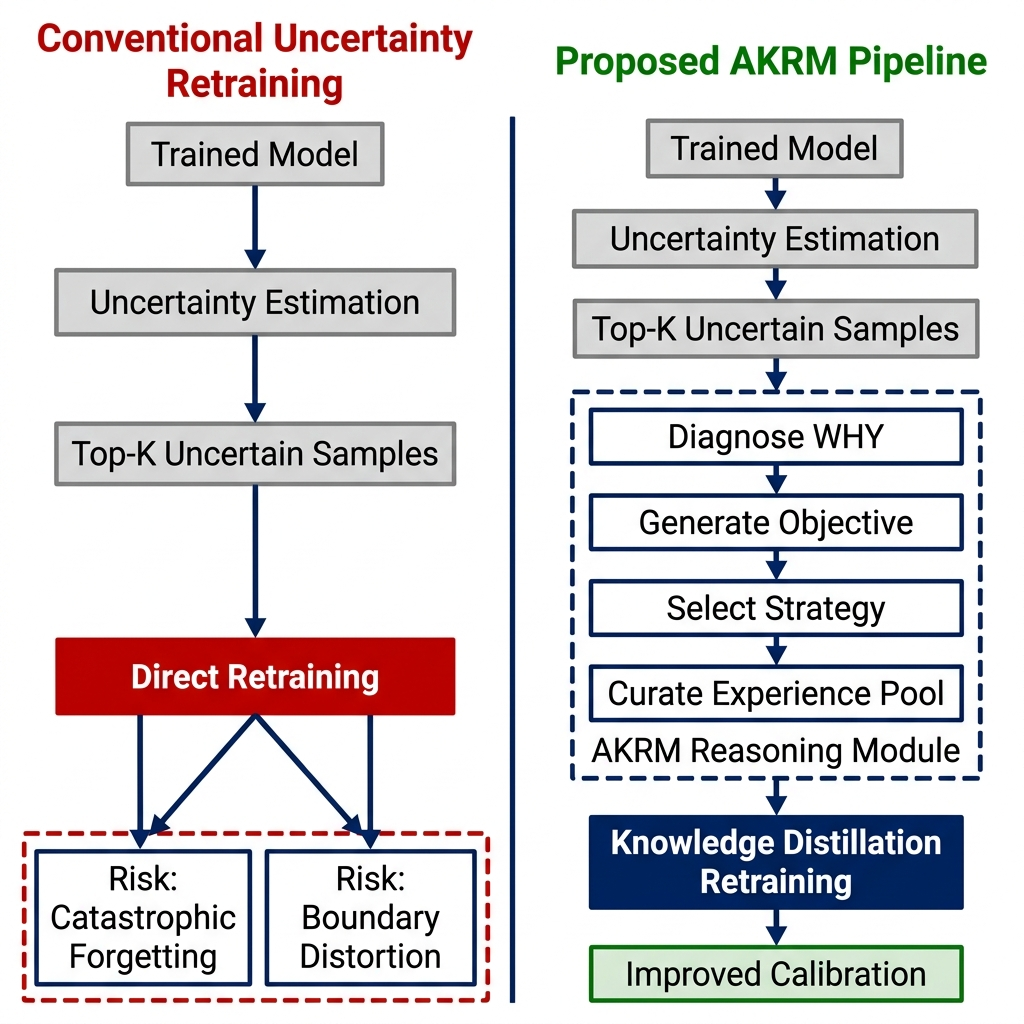
\includegraphics[width=\columnwidth]{figures/figure2_comparison.png}
\caption{Workflow comparison. Left: conventional uncertainty-guided retraining passes uncertain samples directly to training, risking catastrophic forgetting and boundary distortion. Right: proposed AKRM pipeline inserts a structured reasoning phase---\emph{diagnose $\rightarrow$ plan $\rightarrow$ provide $\rightarrow$ retrain}---between uncertainty estimation and learning.}
\label{fig:comparison}
\end{figure}

% ================================================================
% IV. PROPOSED FRAMEWORK
% ================================================================
\section{Proposed Framework}

\subsection{Terminology}

\textbf{Knowledge Gap.} A \emph{knowledge gap} is a localised deficiency in a neural network's learned representation that prevents confident and reliable prediction for a specific region of the input space, despite prior training. Critically, a knowledge gap has a diagnosable \emph{cause}---such as an ambiguous decision boundary or a sparse distributional region---that determines the appropriate corrective action.

\textbf{Reasoning (in AKRM).} The process of transforming raw predictive uncertainty into a structured learning decision through four sequential stages: (i)~diagnosing the cause of uncertainty, (ii)~generating a learning objective, (iii)~planning a data provision strategy, and (iv)~selecting the corrective experience set.

\subsection{Uncertainty Estimation}

MC Dropout~\cite{gal2016dropout} is applied with $T=30$ stochastic forward passes. The per-class mean predictive probability is:
\begin{equation}
\bar{p}_c = \frac{1}{T}\sum_{t=1}^{T} p_c^{(t)}
\end{equation}
and predictive entropy is:
\begin{equation}
H[y \mid x] = -\sum_{c=1}^{C} \bar{p}_c \log \bar{p}_c
\end{equation}
The top $K=10\%$ of samples ranked by $H[y \mid x]$ are forwarded to the AKRM.

\subsection{AKRM Architecture}

The complete pipeline is shown in Fig.~\ref{fig:architecture}. The AKRM intercepts uncertain samples and applies four sequential reasoning steps before any learning occurs.

\begin{figure}[t]
\centering
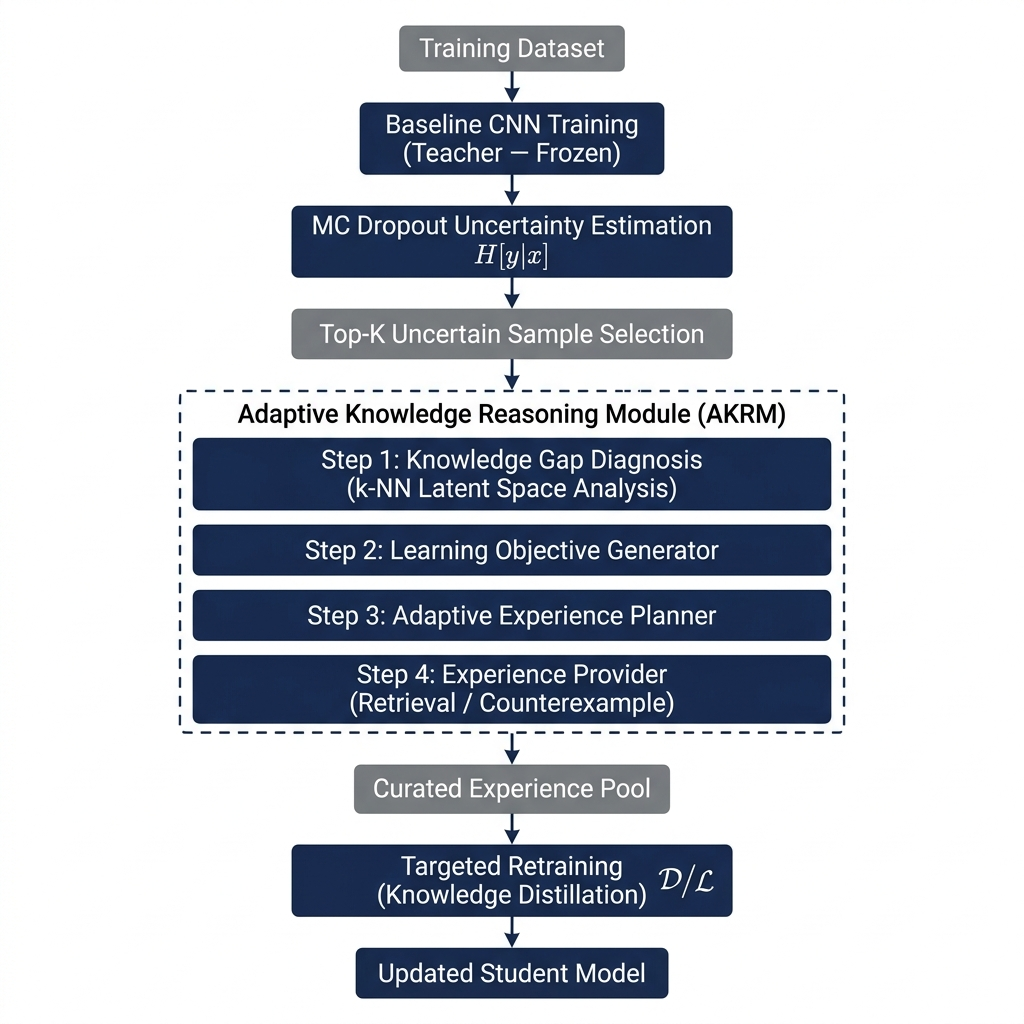
\includegraphics[width=\columnwidth]{figures/figure1_akrm.png}
\caption{Adaptive Knowledge Reasoning Module (AKRM) architecture. The module intercepts uncertain samples after entropy-based selection, performs four-step structured reasoning, assembles a curated Experience Pool, and passes it to teacher-guided distillation retraining.}
\label{fig:architecture}
\end{figure}

The decomposition of AKRM into four discrete components---Knowledge Gap Diagnosis, Learning Objective Generator, Adaptive Experience Planner, and Experience Provider---is intentionally modular. Each component operates on a well-defined input/output contract (e.g., the Diagnoser outputs a gap type; the Planner outputs a strategy identifier; the Provider outputs an index set). This design means that any individual component can be independently improved, replaced, or extended in future work without altering the overall orchestration logic.

\textbf{Step~1---Knowledge Gap Diagnosis.}
Uncertain samples are projected into the latent embedding space (penultimate-layer activations) of the frozen baseline model. A $k$-Nearest Neighbours ($k$-NN) analysis characterises the local geometric structure. $k$-NN is chosen as an initial diagnostic heuristic because it is: (i)~computationally efficient, requiring no additional training; (ii)~interpretable, providing a transparent view of neighbourhood structure; and (iii)~consistent with prior latent-space analysis methods. It is not presented as the theoretically optimal approach. Future work may investigate Mahalanobis distance scoring, density-based outlier detection, graph-based neighbourhood analysis, or learned diagnostic classifiers.

Based on the class composition of the $k$ nearest neighbours, each sample is tentatively assigned one of two initial gap types:
\begin{itemize}
    \item \emph{Boundary Confusion}: the neighbourhood contains a high proportion of samples from a different class, indicating proximity to a poorly defined decision boundary.
    \item \emph{Distributional Anomaly}: the neighbourhood is sparse relative to the training distribution, indicating an underrepresented input type.
\end{itemize}

\textbf{Step~2---Learning Objective Generator.}
Each gap type maps to a structured learning objective. Boundary confusion generates the objective of sharpening the inter-class discriminative boundary; a distributional anomaly generates the objective of improving class-density coverage.

\textbf{Step~3---Adaptive Experience Planner.}
The objective is translated into a data provision strategy. Currently implemented: \emph{Informative Sample Retrieval} (high-confidence samples retrieved to reinforce the correct boundary) and \emph{Counterexample Retrieval} (confident samples from the confused class retrieved to strengthen inter-class separation). Planned: synthetic generation and context-aware augmentation.

\textbf{Step~4---Experience Provider \& Pool Assembly.}
The selected strategy is executed. Retrieved samples are deduplicated and assembled into a curated \emph{Experience Pool}---a targeted data subset addressing the diagnosed knowledge gap.

\textbf{Step~5---Targeted Retraining.}
To prevent catastrophic forgetting, all retraining is performed using a teacher--student distillation scheme~\cite{hinton2015distilling}. The frozen baseline serves as teacher, providing soft output distributions that encode its existing knowledge as a distributional anchor. The dual-loss objective is:
\begin{equation}
\mathcal{L}_{\text{total}} = \alpha \cdot \mathcal{L}_{\text{CE}}(y, \hat{y}) + (1-\alpha) \cdot \mathcal{L}_{\text{KL}}\!\left(\sigma\!\left(\frac{z_T}{\tau}\right), \sigma\!\left(\frac{z_S}{\tau}\right)\right)
\end{equation}
where $\mathcal{L}_{\text{CE}}$ is cross-entropy against ground-truth labels~$y$, $\mathcal{L}_{\text{KL}}$ is the KL-divergence between the frozen teacher's and student's softened logits at temperature $\tau > 1$, and $\alpha \in [0,1]$ balances the two objectives. This formulation is designed to allow the student to learn from the AKRM-curated Experience Pool while the teacher's distributional signal prevents overwriting of previously consolidated representations.

% ================================================================
% V. EXPECTED EVALUATION
% ================================================================
\section{Expected Evaluation}

\textbf{Protocol.}
Full validation is planned on CIFAR-10 and Fashion-MNIST (primary) and CIFAR-100 (scalability). All experiments will use a minimum of 5 independent random seeds. Results will be reported as mean~$\pm$~standard deviation with 95\% confidence intervals. Statistical significance will be assessed using the Wilcoxon signed-rank test. Planned ablations: (i)~no gap diagnosis (random strategy), (ii)~no distillation (standard cross-entropy only), (iii)~no experience planner (uncertain samples retrained directly).

\begin{table}[t]
\centering
\caption{Methodological comparison of existing approaches and the proposed AKRM framework.}
\label{tab:comparison}
\small
\begin{tabular}{@{}lccccc@{}}
\toprule
\textbf{Method} & \textbf{Unc.} & \textbf{Diag.} & \textbf{Adapt.} & \textbf{Forget} & \textbf{Reason.} \\
\midrule
Active Learning~\cite{settles2009active} & \checkmark & -- & -- & -- & -- \\
MC Retraining~\cite{gal2016dropout} & \checkmark & -- & -- & -- & -- \\
EWC~\cite{kirkpatrick2017overcoming} & -- & -- & -- & \checkmark & -- \\
Distillation~\cite{hinton2015distilling} & -- & -- & -- & \checkmark & -- \\
\textbf{Proposed AKRM} & \checkmark & \checkmark & \checkmark & \checkmark & \checkmark \\
\bottomrule
\end{tabular}
\end{table}

% ================================================================
% VI. DISCUSSION, LIMITATIONS & FUTURE WORK
% ================================================================
\section{Discussion, Limitations \& Future Work}

\textbf{Central Insight.}
Predictive uncertainty is a symptom of a knowledge gap, not a diagnosis of its cause. AKRM is designed to treat the cause by reasoning about \emph{why} the model is uncertain before selecting a calibrated corrective action.

\textbf{Limitations.}
We explicitly acknowledge: (i)~\emph{Heuristic diagnosis}---the $k$-NN analysis is an initial heuristic; diagnosis errors may lead to misaligned strategy selection, potentially compounding rather than correcting the model's deficiency. (ii)~\emph{Representation dependence}---diagnostic quality is bounded by the baseline model's latent structure; if the penultimate-layer representations are poorly organised, the $k$-NN neighbourhood may not reflect the true nature of the gap. (iii)~\emph{Computational overhead}---embedding extraction, $k$-NN search, and pool assembly introduce cost not present in direct retraining. (iv)~\emph{Coarse taxonomy}---the current two-type taxonomy (boundary confusion vs.\ distributional anomaly) does not capture label noise, class imbalance, or distributional shift. (v)~\emph{Scalability}---the framework has not yet been evaluated on large-scale datasets or deep architectures.

\textbf{Future Work.}
Planned extensions include: probabilistic gap diagnosis (Mahalanobis distance, density estimation), a finer-grained knowledge gap taxonomy, a knowledge memory cache to reduce redundant computation, dynamic adaptation of~$\tau$ and~$\alpha$ based on diagnosed gap severity, and evaluation on CIFAR-100, ImageNet subsets, and Vision Transformer backbones.

% ================================================================
% VII. CONCLUSION
% ================================================================
\section{Conclusion}

We have presented AKRM, an early-stage framework proposal for reasoning-driven, uncertainty-aware neural network retraining. Motivated by preliminary observations that blind uncertainty-guided retraining can degrade model performance through catastrophic forgetting and boundary distortion, AKRM is designed to diagnose the \emph{cause} of predictive uncertainty in latent space before selecting a targeted corrective learning strategy. Teacher-guided distillation is incorporated as a first-class forgetting-prevention constraint. The framework's conceptual contribution---separating \emph{``which samples are uncertain?''} from \emph{``why are they uncertain?''} and \emph{``how should the model learn?''}---represents a new research direction toward principled, reasoning-driven uncertainty-aware continual learning.

% ================================================================
% REFERENCES
% ================================================================
\begin{thebibliography}{9}
\bibitem{gal2016dropout}
Y.~Gal and Z.~Ghahramani, ``Dropout as a {B}ayesian Approximation: Representing Model Uncertainty in Deep Learning,'' in \emph{Proc. ICML}, vol.~48, pp.~1050--1059, 2016.

\bibitem{lakshminarayanan2017simple}
B.~Lakshminarayanan, A.~Pritzel, and C.~Blundell, ``Simple and Scalable Predictive Uncertainty Estimation using Deep Ensembles,'' in \emph{Adv. NeurIPS}, vol.~30, pp.~6402--6413, 2017.

\bibitem{settles2009active}
B.~Settles, ``Active Learning Literature Survey,'' Tech. Rep.~1648, Univ.\ of Wisconsin--Madison, 2009.

\bibitem{kirkpatrick2017overcoming}
J.~Kirkpatrick \emph{et al.}, ``Overcoming Catastrophic Forgetting in Neural Networks,'' \emph{PNAS}, vol.~114, no.~13, pp.~3521--3526, 2017.

\bibitem{hinton2015distilling}
G.~Hinton, O.~Vinyals, and J.~Dean, ``Distilling the Knowledge in a Neural Network,'' \emph{arXiv:1503.02531}, 2015.

\bibitem{nguyen2015fooled}
A.~Nguyen, J.~Yosinski, and J.~Clune, ``Deep Neural Networks are Easily Fooled,'' in \emph{Proc. CVPR}, pp.~427--436, 2015.

\bibitem{guo2017calibration}
C.~Guo, G.~Pleiss, Y.~Sun, and K.~Q.~Weinberger, ``On Calibration of Modern Neural Networks,'' in \emph{Proc. ICML}, vol.~70, pp.~1321--1330, 2017.

\bibitem{gawlikowski2023survey}
J.~Gawlikowski \emph{et al.}, ``A Survey of Uncertainty in Deep Neural Networks,'' \emph{Artif. Intell. Rev.}, vol.~56, Suppl.~1, pp.~1513--1589, 2023.

\bibitem{wang2024epistemic}
H.~Wang and Q.~Ji, ``Epistemic Uncertainty Quantification for Pre-trained Neural Networks,'' in \emph{Proc. CVPR}, 2024.
\end{thebibliography}

\end{document}
